\documentclass{article}
\usepackage[T1]{fontenc}
\usepackage{a4wide}
\usepackage{times}
\usepackage{listings}
\usepackage{url}

%% TeXcount parsing rules
%TC:envir lstlisting [] xall
%TC:macro url [ignore]

%% LaTeX macros
\usepackage{relsize}
\usepackage[dvipsnames]{xcolor}

% Define underscore to be a regular character in text mode
\begingroup
  \catcode`\_=\active
  \gdef_#1{\ensuremath{\sb{#1}}}
\endgroup
\mathcode`\_=\string"8000
\catcode`\_=12

% Set version number
\newcommand\version{$3.0$}

\newcommand\copyrightfootnote{
\footnotetext{Copyright (2008-2013) of Einar Andreas R{\o}dland, distributed
under the \LaTeX{} Project Public License (LPPL).}
}

%TC:macroword \TeXcount 1
\newcommand\TeXcount{{\TeX}count}

% Text formats
\newcommand\codestyle[1]{\textsf{\color{Blue}#1}}
\newcommand\code[1]{{\smaller\codestyle{#1}}}
\newcommand\bigcode[1]{\codestyle{#1}}
\newcommand\codeline[1]{\begin{quote}\code{#1}\end{quote}}
\newcommand\bs[1]{\textbackslash#1}
\newcommand\URL[1]{\textsf{\small #1}}

% Description items: options, parameters, optional parameters
% These are also interpreted by dos2html.pl
\def\option[#1]{\item[\bigcode{#1}]\hskip 0pt plus 10pt}
\def\parm#1{\textit{\color{OliveGreen}#1}}
\def\opt#1{\parm{[#1]}}
\def\alt#1{[#1]}
\def\optiontext#1{\textrm{\bfseries\color{black}#1}}

% Mark off notification in contents for good visibility
\newcommand\ContentsNote[1]{\addtocontents{toc}{\string\marginpar{\textsf{\color{red}\tiny #1}}}}

% Notabene: margin note
%TC:macro NB 1
\newcommand\NB[1]{\ContentsNote{NB}\marginpar{\textsf{\tiny#1}}}

% Mark text as a notification
%TC:macro NOTE [text]
\newcommand\NOTE[1]{\textit{\color{red}#1}}

% Mark text for update
%TC:macro UPDATE [text]
\newcommand\UPDATE[1]{\ContentsNote{UPDATE}\textit{\textbf{\color{red}This needs to be updated:} {\color{blue}#1}}}

% Mark text as a notification
%TC:macro TODO [text]
\newcommand\TODO[1]{\ContentsNote{TODO}\textit{\textbf{\color{red}#1}}}

% BUG
%TC:macro BUG [text]
\newcommand\BUG[1]{{\color{red}#1}}

\makeatletter

\renewcommand\@maketitle{%
\newpage\null\vskip 2em%
\begin{center}%
\let\footnote\thanks
{\LARGE \@title \par}%
\end{center}%
\par
\vskip 1.5em
}

\renewcommand\abstractname{Abstract}
\renewenvironment{abstract}{%
  \begin{center}%
    {\slshape\bfseries\large\abstractname\vspace{-.5em}\vspace{\z@}}%
  \end{center}%
  \vskip 4pt
  \slshape
}{
\vskip 0.5em
}

\makeatother


%\parindent=0pt\parskip=8pt
\lstset{basicstyle=\ttfamily\scriptsize,xleftmargin=2cm,xrightmargin=2cm}
\lstset{basicstyle=\ttfamily\scriptsize,xleftmargin=2cm,xrightmargin=2cm}

\title{%
\LARGE
\TeXcount\\
\Large
Perl script for counting words in \LaTeX{} documents\\
Version \version\copyrightfootnote
}
\author{Einar Andreas R{\o}dland}

\begin{document}

\maketitle

{\abstract%
\TeXcount{} is a Perl script for counting words in \LaTeX{} documents. It recognises most of the common macros, and has rules for which parameters to count and not to count; the main text is counted separately from the words in headers and in captions of figures and tables. Finally, it produces a colour coded version of the parsed document, either as a text document or as HTML to be viewed in a browser, indicating which parts of the document have been included in the count.
%
}

{\scriptsize\tableofcontents}

\pagebreak


% ---------------------------------------------------------------------------

\section{What \TeXcount{} does}

\TeXcount{} is a Perl script made for counting the words in a \LaTeX{} document. Since \LaTeX{} documents are formated using lots of macro instructions and often contain both mathematical formulae and floating tables and figures, this is no trivial task.

Simple solutions to counting the words consists of detexing the documents, which often merely consisty of ignoring the \TeX{} and \LaTeX{} instructions. This is a bad solution since it will usually result in over-estimating the number of words as mathematical formulae, citations, labels and references are counted.

A perfect solution, if such exists, needs to take into account how \LaTeX{} interprets each macro instruction. The simplest approach to taking this into account consisty of making the count based on the typeset document, but this too tends to over-estimate the word count as mathematical formulae, table contents and even page numbers may get counted.

A simple but robust approach, which is the one I have taken with \TeXcount{}, is to parse the \LaTeX{} document using simple rules for how to interpret the different \TeX{} and \LaTeX{} instructions. Rules for most of the common macro instructions are included in \TeXcount{}, and it is possible to specify new rules in the \TeX{} document.

The primary focus of \TeXcount{} is to:
\begin{itemize}

\item provide an accurate count of the number of words in \LaTeX documents;

\item exclude or count separately document elements which are not part of the main text such as figure captions;

\item enable the user to, with relative ease, check how \TeXcount{} has parsed the document and which elements have been counted and which have not.

\end{itemize}
The last point on this list is one of the most important. Having an accurate word count is of little value unless you know that it is accurate; conversly, trusting an inaccurate word count can be potentially harmful, e.g. if you are submitting a paper or a report which has a strict word limit.

\TeXcount{} handles complete \LaTeX{} documents, i.e. that start with \code{\bs{documentclass}} and has the text between \code{\bs{begin}\{document\}} and \code{\bs{end}\{document\}}, as well as partial documents made to be included in another \LaTeX{} document. However, in either case, it requires that all groups are closed: \code{\{\ldots\}} and \code{\bs{begin}\ldots\bs{end}}.

Automatic parsing of included documents is possible, but is by default turned off. There are two options for turning this on: \code{-inc} and \code{-merge}. Turning it on using \code{-merge} will merge the included files into the main document. By using \code{-inc}, however, the included files are parsed separately rather than include the text into the appropriate location: this will perform a separate word count of the included document which is then later included in the total sum.

Since \TeXcount{} relies on a relatively simple rules for handling the different macros and only performs limited checks on the validity of the \LaTeX{} document, it is your responsibility to make sure the document actually typesets in \LaTeX{} before running it through \TeXcount{}. Also, \TeXcount{} relies on handling macros taking parameters enclosed with \{ and \}, and on ignoring options enclosed by [ and ]: macros with significantly different syntax such as \code{\bs{vskip}} cannot be handled. There are also limitations on what may be contained in macro options enclosed in [], although this restriction may be relaxed by specifying the command line option \code{-relaxed}.


\subsection{What \TeXcount{} counts}

Basically, \TeXcount{} has seven different counts plus an additional file count for use with total counts over a set of files. These and their indices (numbers used to identify them) are:
\begin{description}
\item[0. Number of files:] When multiple files are included, this is counted.
\item[1. Text words:] Words that occur in the main text.
\item[2. Header words:] Words that occur in headers, e.g. \code{\bs{title}} and \code{\bs{section}}.
\item[3. Caption words:] Words that occur in figure and table captions.
\item[4. Header count:] This counts the number of headers, i.e. each \code{\bs{section}} counts as 1.
\item[5. Figure/float count:] This counts the number of floats and figures, e.g. \code{table} and \code{figure} environments.
\item[6. Inline formulae:] This counts the number of inline formulae, i.e. \code{\$\ldots\$}.
\item[7. Displayed formulae:] This counts the number of displayed formulae, e.g. \code{\bs{[}\ldots\bs{]}} or \code{equation} environments.
\end{description}
These are stored in an array and sometimes referenced by their index: e.g. in the option \code{-sum=} which takes parameter values corresponding to counts 1 to 7. In other contexts, however, like in the \code{-tempate=} or when incrementing specific counters through the \code{\%TC:macrocount} instruction, the counters may be referred to by keywords rather than the indices 0 to 7.

The primary role is to count the words. It is not entirely clear what should be considered words, so I have had to make some decisions. A sequence of letters is certainly a word. \TeXcount{} also counts acronyms like \textit{e.g.}, dashed words like \textit{over-all}, and \textit{it's} as one word. It also counts numbers as words unless they are placed in a math group. If \TeXcount{} breaks words that contain special characters, you may try the option \code{-relaxed} which extends the range of characters allowed as part of words.

Alternatively, \TeXcount{} may be asked to count the number of letters/characters (not including spaces). It may also be set to count Chinese or Japanese characters.

Mathematical formulae are not counted as words: it would be difficult to define a sensible rule for this. Instead, \TeXcount{} counts the number of inline formulae and displayed formulae separately. You may then decide on how to combine these counts with the word counts, e.g. using the \code{-sum} option.

Text in headers (\code{\bs{title}}, \code{\bs{section}}, etc.) are counted separately: \TeXcount{} counts the number of headers as well as the number of words in headers. It may also provide subcounts for each of these by specifying the \code{-sub} option.

Floating environments (or potentially floating environments) such as tables and figures are not counted as text, even if the cells of a table may containt text. However, if they have captions, these will be counted separately much like headers were. Footnotes are included in this count. By default, environments do not modify the parsing state: i.e. environments within the text are counted as text, etc. Rules for the most common environments, at least those that require non-default treatment, should be predefined, but you may have to add more rules if you use environments defined in packages or by yourself. If you wish to be warned against any environments names you use that lack a defined rule, set the option \code{-strict}.

Some macros are words by themselves: e.g. \code{\bs{LaTeX}}. These are counted as words provided the macro word rule has been defined for them, but you cannot expect \TeXcount{} to count something like \code{\bs{LaTeX}-word} or \code{\{\bs{TeX}\}count} as one word although the above explanation inicates that it should: \TeXcount{} will in both cases evaluate the macro and the following text separately and thus count them as separate entities. Since \TeXcount{} recognises \code{\bs{LaTeX}} and \code{\bs{TeX}} as single words, each of the two examples would end up being counted as two words.


\subsection{What \TeXcount{} does not do}

While an ideal solution should be able to expand the macro instructions, thus being able to handle new macros, that would at it's worst require reimplementing much of \TeX{}, something that is clearly unrealistic. Instead, I have opted for a simpler solution: to define rules stating which paramters to count and which to ignore and allowing for such rules to be added easily. Thus, \TeXcount{} cannot handle macros that may take a variable number of parameters. Nor can it handle macros that takes parameters on forms other than \code{\{parameter\}}. However, support has now been added for macro options on the form \code{[\ldots]} to be parsed.

In general, while \TeXcount{} does the parsing in some detail, it does not do it exacly as \TeX{} does it. In some respects there may therefore be critical differences: e.g. while \TeX{} reads one character at a time, \TeXcount{} reads one word at a time, so while \LaTeX{} would interpret \code{\bs{cite} me} as \code{\bs{}cite\{m\}e}, \TeXcount{} would interpret it like \code{\bs{cite}\{me\}}.

Another issue is that, since \TeXcount{} does not know how to expand macros, it cannot handle macros like \code{\bs{maketitle}} that add text to the document. With respect to \code{\bs{maketitle}}, I have instead set the rule for \code{\bs{title}\{title text\}} to count this as a header although it does not itself produce any text.


\subsection{Problems to be aware of}

In most large documents, there will be cases where \TeXcount{} does not give an exact count. Reasons may be macros \TeXcount{} does not recognise, words that \TeXcount{} split in two (or more) because of special characters not recognised as letters, or options and parameters not counted which actually produce text. Some problems may also arise because it is not always clear what should be counted and \TeXcount{} implements one particular choice: counting numbers as letters/words, not counting formulae as words, not to count tables as text, etc. However, hopefully these should either consist of individual, infrequent errors which should have limited effect on the total count, or entire regions that are included or excluded for which the user may change the parsing rule to produce the desired count.

There are, however, problems that may arise which are more fundamental and result in counts which are simply wrong rather than just inaccurate, or even make \TeXcount{} fail entirely.

If \TeXcount{} fails to detect environment endings properly, either closing \code{\{} or \code{\bs{end}}, it may end up ignoring major parts of the document. This should normally produce errors of some kind, although there may be cases when no errors are produced. However, by looking at the verbose output, it will be very clear that entire parts of the document has been excluded. Such problems may be cause by macros that allow unmatched group delimiters, and some effort has been made to minimise the risk of this at the cost of risking other but less critical errors: e.g. there are limits to what is permitted as macro options in order to ensure that a single unmatched \code{[} does not cause large parts of the document to be interpreted as a big option.

For users of languages containing letters other than the Latin letters A to Z, there is a risk that \TeXcount{} may have difficulty identifying words correctly. The script relies on Perl to recognise words as sequence of letters, and must therefore know which characters are considered to be letters. Words containing letters not recognised by \TeXcount{} will tend to be split into two or more words, which can dramatically inflate the word count. The first step is to ensure that the file is read using the correct encoding: I generally suggest using the UTF-8 Unicode encoding, and from version 2.3. this is the default encoding used by \TeXcount{}, although other encodings may also be used. Unicode has good annotation of which characters are letters, and starting with version 2.3, \TeXcount{} uses Unicode internally to represent the text.

While non-Latin letters like \code{\aa} and \code{\"a} should be recognised as letters, \TeX/\LaTeX codes using macros or special characters, such as \code{\bs{aa}} and \code{\bs{"}a}, are not immediately understood as letters. I have added patterns aimed at recognising these as well, but depending on the code you are writing, these patterns may either not be flexible enough to recognise all letter codes, or may be too flexible and recognise things it should not. I have added a relaxed mode (\code{-relaxed}) and a more restricted mode (\code{-restricted}) in which these patterns are more general or more constrained, but you should check how this performs on you actual texts by viewing the verbose output.



% ---------------------------------------------------------------------------

\section{Syntax and options}


\subsection{Running \TeXcount{}}

The command to run \TeXcount{} may vary slightly depending on the operating system and the local settings. You may also wish to rename it or define an alias.

Under Windows, running \code{texcount.pl} from the command line suffices if \code{texcount.pl} is in the path and pl-files are defined to run as Perl scripts.

Under Linux/Unix, it should be sufficient to run \code{texcount.pl} provided it is in the PATH and has been made executable (\code{chmod u+x texcount.pl}). The first line of the file contains the line \code{\#!/usr/bin/env perl} which should find the correct location for \code{perl} (provided the program \code{/usr/bin/env} is available). If not, run \code{which perl} to locate Perl and replace the first line of the script with \code{\#!\textit{path}}.

Alternatively, if the above methods do not work, you may have to run \TeXcount{} exclicitly in Perl by executing \code{perl texcount.pl}. You then need to have the \code{perl} executable in the path or give the explicit path.

For simplicity, I will simply write \code{texcount.pl} in this manual for the code to execute the script. The syntax then becomes
\codeline{texcount.pl \textit{[options] [files]}}
where the options may be amongst the following:

% Subsection: command line options

\begin{description}
\sloppy
\def\option[#1]{\item[\quad\code{#1}]\hskip 0pt plus 10pt}
\def\alt#1{[#1]}
\def\alts#1{[[#1]]}

\option[-v]Verbose (same as \code{-v3}).

\option[-v0]No details (default).

\option[-v1]Prints counted text, marks formulae.

\option[-v2]Also prints ignored text.

\option[-v3]Also includes comments and options.

\option[-v4]Same as \code{-v3 -showstate}.

\option[-v=\ldots, -v\alts{0-4}\ldots]Allows detailed control of which elements are included in the verbose output. The provided values is a list of styles or style categories separated by \code{+} or \code{-} to indicate if they should be added or removed from the list of included styles. Style categories start with capital letter and include \code{Words}, \code{Macros}, \code{Options}; the individual styles are in all lower case and include \code{word}, \code{hword}, \code{option}, \code{ignore}.

\option[-showstate]Show internal states (with verbose).

\option[-brief]Only prints a one line summary of the counts for each file.

\option[-q, -quiet]Quiet mode, does not print error messages. Use is discouraged, but it may be useful when piping the output into another application.

\option[-strict]Prints a warning of begin-end groups for which no specific rule is defined.

\option[-total]Only give total sum, no per file sums.

\option[-1]Same as specifying \code{-brief} and \code{-total}, and ensures there will only be one line of output. If used with \code{-sum}, the output will only be the total number.

\option[-0]Same as \code{-1}, i.e. \code{-brief} and \code{-total}, but does not put a line shift at the end. This may be useful when the one line output is to be used by another application, e.g. Emacs, for which the line shift would otherwise need to be stripped away.

\option[-template="\ldots"]Specify an output template which is used to generate the summary output for each file and for the total count. Codes \code{\{\textit{label}\}} is used to include values, where \code{\textit{label}} is one of \code{0} to \code{7} (for the counts), \code{SUM}, \code{ERROR} or \code{TITLE} (first character of label is sufficient). Conditional inclusion is done using \code{\{\textit{label}?\textit{text}?\textit{label}\}} or \code{\{\textit{label}?\textit{if non-zero}|\textit{if zero}?\textit{label}\}}. If the count contains at least two subcounts, use \code{\{SUB|\textit{template}|SUB\}} with a separate template for the subcounts, or \code{\{SUB?\textit{prefix}|\textit{template}|\textit{suffix}?SUB\}}.

\option[-sub\alt{=\ldots}, -subcount\alt{=\ldots}]Generate subcounts. Valid option values are \code{none}, \code{part}, \code{chapter}, \code{section} and \code{subsection} (default), indicating at which level subcounts are generated. (On by default.)

\option[-nosub]Do not generate subcounts.

\option[-sum\alt{=n,n,\ldots}]Produces total sum, default being all words and formulae, but customisable to any weighted sum of the seven counts (list of weights for text words, header words, caption words, headers, floats, inlined formulae, displayed formulae).

\option[-nosum]Do not generate total sum. (Default choice.)

\option[-col]Use ANSI colour codes in verbose output. This requires ANSI colours which is used on Linux, but may not be available under Windows. On by default on non-Windows systems. 

\option[-nc, -nocol]No colours (colours require ANSI). Default under Windows.

\option[-nosep, -noseparator]No separating character/string added after each word in the verbose output (default).

\option[-sep=, -separator=]Separating character or string to be added after each word in the verbose output.

\option[-relaxed]Relaxes the rules for matching words and macro options.

\option[-restricted]Restricts the rules for matching words and macro options.

\option[-]Read \LaTeX{} code from STDIN.

\option[-inc]Parse included files (as separate files).

\option[-merge]Merge included files into document (in place).

\option[-noinc]Do not parse or merge in included files (default).

\option[-incbib]Include bibliography in count, include bbl file if needed.

\option[-nobib]Do not include bibliography in count (default).

\option[-incpackage=]Include rules for a given package.

\option[-dir\alt{=\ldots}]Specify working directory which will serve as root for all include files. The default (\code{-dir=.}) is to use the current directory, i.e. from which \TeXcount{} is executed: the path can be absolute or relative to the current directory. Use \code{-dir} to use the path of the main \LaTeX{} document as working directory.

\option[-auxdir\alt{=\ldots}]Specify the directory of the auxiliary files, e.g. the bibliography (\code{.bbl}) file. The default setting (\code{-auxdir} only) indicates that auxiliary files are in the working directory (from the \code{-dir} or \code{-dir=} option). If \code{-auxdir=} is used to provide a path and \code{-dir=} is used to specify the working directory, the path to the auxiliary directory is take to be relative to the current folder (from which \TeXcount{} is executed); if used with \code{-dir}, the working directory is taken from the path of the parsed file, and the auxiliary directory is taken to be relative to this (unless an absolute path is provided).

\option[-enc=, -encoding=]Specify encoding to use in input (and text output).

\option[-utf8, -unicode]Use UTF-8 (Unicode) encoding. Same as \code{-encoding=utf8}.

\option[-alpha=, -alphabets=]List of Unicode character groups (or digit, alphabetic) permitted as letters. Names are separated by \code{,} or \code{+}. If list starts with \code{+}, the alphabets will be added to those already included. The default is Digit+alphabetic.

\option[-logo=, -logograms=]List of Unicode character groups interpreted as whole word characters, e.g. Han for Chinese characters. Names are separated by \code{,} or \code{+}. If list starts with \code{+}, the alphabets will be added to those already included. By default, this is set to include Ideographic, Katakana, Hiragana, Thai and Lao.

\option[-ch, -chinese, -zhongwen]Turn on Chinese mode in which Chinese characters are counted. I recommend using UTF-8, although \TeXcount{} will also test other encodings (GB2312, Big5, Hz) if UTF-8 fails, and other encodings may be specified by \code{-encoding=}.

\option[-jp, -japanese]Turn on Japanese mode in which Japanese characters (Kanji and Kana) are counted. I recommend using UTF-8, although \TeXcount{} will also test other encodings (e.g. EUC-JP) if UTF-8 fails, and other encodings may be specified by \code{-encoding=}.

\option[-kr, -korean]Turn on Korean mode in which Korean characters (Hangul and Han) are counted. I recommend using UTF-8, although \TeXcount{} will also test other encodings (e.g. EUC-KR) if UTF-8 fails, and other encodings may be specified by \code{-encoding=}.

\option[-kr-words, -korean-words]Korean mode in which Hangul words are counted (i.e. as words separated by spaces) rather than characters. Han characters are still counted as characters. See also \code{-korean}.

\option[-chinese-only, ..., -korean-words-only]As options \code{-chinese}, ..., \code{-korean-words}, but also excludes other alphabets (e.g. letter-based words) and logographic characters.

\option[-char, -letter]Count letters instead of words. This count does not include spaces.

\option[-out=]Send output to file. Takes file name as value.

\option[-html]Output in HTML format.

\option[-htmlcore]Only HTML body contents.

\option[-htmlfile=]File containing a template HTML document with \code{<!-- TeXcount -->} included somewhere to indicate the location where the TeXcount output from the parsing should be inserted.

\option[-tex]Encode \TeX{} special characters for output into \TeX{} code.

\option[-css=]Reference to CSS to be included in the HTML output instead of including the style definition directly in the output.

\option[-cssfile=, -css=file:]File containing style definitions to be included into the HTML output instead of the default styles.

\option[-freq\alt{=\#}]Count individual word frequencies. Optionally, give minimal frequency required to be included in output.

\option[-stat]Produce statistics on language usage, i.e. based on the alphabets and logograms included.

\option[-macrostat, -macrofreq]Produce statistics on package, environment and macro usage. 

\option[-codes]Display an overview of the colour codes. Can be used as a separate option to only display the colour codes, or together with files to parse.

\option[-nocodes]Do not display overview of colour codes.

\option[-opt=, -optionfile=]Reads options (command line parameters) from a specified text file. Should use one option per line. May also include TC options in the same format as specified in \LaTeX{} documents, but prefixed by \code{\%} rather than \code{\%TC:}. Blank lines and lines starting with \code{\#} are ignored; lines starting with \code{\bs{}} are considered to be continuations of the previous line.

\option[-split, -nosplit]The \code{-split} option, which is on by default, speeds up handling of large files by splitting the file into paragraphs. To turn it off, use the \code{-nosplit} option.

\option[-showver, -nover]Include version number in output with \code{-showver}; use \code{-nover} not to show it (default). 

\option[-h, -?, --help, /?]Help.

\option[-h=, -?=, --help=, /?=]Help on particular macro or group name: gives the parsing rule for that macro or group if defined. If the the macro or environment is package specific, use \code{-h=\parm{package}:\parm{name}}; replace \code{\parm{package}} with \code{class\%\parm{name}} if it is specific to a document class.

\option[-help-options, -h-opt]Lists all TeXcount options and help on them.

\option[--help-option=, -h-opt=]Lists all TeXcount options containing the provided string: e.g. \code{-h-opt=inc} lists all options containing \code{inc}, while \code{-h-opt=-v} lists all options starting with \code{v}.

\option[-help-style, -h-style]Lists all styles and style categories, i.e. those permitted used in -v={styles-list}.

\option[-help-style=, -h-style=]Gives description of style or style category. 

\option[-ver, --version]Print version number.

\option[-lic, --license]License information.

\end{description}


If more than one file is given, \TeXcount{} will perform the count on each of them printing the results for each, then print the total sum at the end. Note that files are parsed one by one in order of appearance and counts made per file; only afterwards are the totals computed. 


\subsection{File encoding}

If your \TeX/\LaTeX{} document consists entirely of ASCII characters, there should be no problems with file encoding. However, if it contains non-ASCII characters, e.g. non-Latin letters such as \o{}, there are different ways in which these may be encoded in the files.

The main encoding supported by \TeXcount{} is UTF-8 (Unicode), and this is used to represent text internally in \TeXcount{}. In older versions of \TeXcount{}, Latin-1 (ISO-8859-1) was the default encoding, but this may cause problems when using non-Latin characters.%
\footnote{%
In Perl, which \TeXcount{} is written in, Latin-1 is the default. However, starting with version 2.3, \TeXcount{} has switched to using UTF-8 (Unicode) internally and will convert text to Unicode before processing: in older version, internal representation was UTF-8 or Latin-1 depending on the options used.}
Both of these are compatible with ASCII: i.e. both are extensions of ASCII, so ASCII characters will be treated correctly by both encodings, but non-ASCII characters will be treated differently.

From version 2.3 of \TeXcount{}, it is possible to specify other encodings using the \code{-encoding=} option. If no encoding is specified, \TeXcount{} will guess which encoding is used. By default, this guessing is limited to ASCII, UTF-8 and Latin-1. If other encodings are used, the automatic guessing is likely to pick Latin-1 since most files would result in valid Latin-1 code. If the \code{-chinese} or \code{-japanese} option is set, it will guess at other encodings, but still with UTF-8 as the first choice.

I generally recommend using UTF-8 Unicode: this is increasingly being the new standard. Basically, Unicode contains the characters needed for all existing languages, enumerated from 0 and upwards (beyond 100000), which resolves to problem of requiring different character sets. Since there are more than 256 characters in Unicode, Unicode cannot be represented using one byte per character: UTF-8 is a way to encode the Unicode characters into a list of bytes so that ASCII characters (no. 0--127) are represented by one byte (same as in ASCII), while non-ASCII characters are represented using two or more bytes. Unicode may also be encoded using two bytes to represent each of Unicode characters 0--65535, which covers most of practical use, but this is less commonly used as a file format: it is, however, common for internal representation of strings in memory, as done by e.g. Java, so Perl is the odd one out in using UTF-8 for internal string representation.

If an encoding is specified using the \code{-encoding=} option, the input will be decoded from the specified encoding into UTF-8. If HTML output is specified, the output will be UTF-8. This ensures that all HTML produced is UTF-8, which is also the encoding specified in the HTML header. If text output is used, the specified encoding is used for the output. E.g. if you specify \code{-encoding=latin1}, \TeXcount{} will assume that all files are encoded in Latin-1, and will also produce the detailed output using Latin-1. For piping, i.e. option \code{-}, this is useful as it ensures the output has the same encoding as the input.

For convenience, if no encoding is specified, \TeXcount{} will try to guess which encoding is the appropriate one. This is done simply by checking a specified list of encodings one by one until one is found that fits the text. The default is to check ASCII, then UTF-8, and finally Latin-1. If none fits, \TeXcount{} should try to decode the ASCII part of the text replacing non-ASCII characters with a wildcard character, although there may be cases when the decoding exits upon hitting an error. If Chinese or Japanese languages are specified, UTF-8 is tried first, then other encodings are checked depending on the language.

Note that if no encoding is specified and \TeXcount{} left to guess the appropriate encoding, all output will be UTF-8. Thus, letting \TeXcount{} guess the encoding may not be suitable when using \TeXcount{} in a pipe since the UTF-8 output may not be compatible with the encoding of the input. If multiple files are parsed, \TeXcount{} will guess the encoding separately for each file even if they are included (\code{-inc} or \code{-merge}) in a file with an identified encoding, and may thus end up selecting different encodings for different files.


\subsection{Language scripts, alphabets and character sets}

In additional to the traditional Latin letters, A-Z, a number of letters are recognised by Unicode as part of the extension of the Latin letters. Some languages, however, use entirely different character sets.

By default, \TeXcount{} has been set up to recognise all alphabets. However, there is a distinction between alphabets like the Latin, Greek, Cyrillic, etc. in which words consists of multiple letters, and languages like Chinese in which each character should be counted as a word. For simplicity, we refer to these as \emph{alphabetic} characters and \emph{logograms}.\footnote{%
Actually, these names are not completely accurate. A logogram is a script which represents a word or `meaningful unit', but e.g. the Japanese kana and Korean hangul are counted as words although they represent sound or syllables rather than meanings.}
The options \code{-alphabets=} and \code{-logograms=} (or \code{-alpha=} and \code{-logo=} for short) allows you to specify which characters to use as either alphabetic letters or whole word characters. These take values that consist of Unicode properties separated by \code{,} or \code{+}. The default setting corresponds to
\codeline{-alphabets=Digit,alphabetic}
in which \code{alphabetic} is defined by \TeXcount{} as the Unicode \code{Alphabetic} class minus logographic script classes, and
\codeline{-logograms=Ideographic,Hiragana,Katakana,Thai,Lao}
which should cover Chinese characters (\code{Han}) as well as the Japanese characters (\code{Han} for the kanji, \code{Hiragana} and \code{Katakana} for the kana). Both options remove previous script settings, unless the list is prefixed by \code{+} in which case the scripts are added: e.g. \code{-logograms=+cjkpunctuation} will add the CJK punctuation characters (defined by \TeXcount) to the set of counted characters.

Applicable Unicode properties/scripts include \code{Digit}, \code{Latin}, \code{Greek}, \code{Cyrillic}, \code{Hebrew}, \code{Arabic}, \code{Han}, \code{Katakana}, \code{Hiragana}, and more.\footnote{A more complete overview is available at Wikipedia: \url{http://en.wikipedia.org/wiki/Script_(Unicode)}.}

In addition to the Unicode properties, \TeXcount{} has added a few additional character groups. The properties \code{alphabetic}, \code{digit} and \code{alphanumeric} are more restrictive than their Unicode name-sakes: \code{alphabetic} excludes the default logographic character sets, and \code{digit} consists only of 0--9 unlike Unicode \code{Digit} which includes numerals from other scripts. There is also \code{cjkpunctuation} which is intended to identify Chinese/Japanese/Korean punctuation.

Note that the Unicode properties are case sensitive. The native Unicode properties start with capital letters, whereas the properties defined by \TeXcount{} are all lower case. Invalid properties will be ignored.

The options \code{-chinese} and \code{-japanese} still exist and simply restrict the logographic character sets. In addition, \code{-chinese-only} and \code{-japanese-only} will exclude alphabetic words from the counting, equivalent to \code{-alphabets=} with no script properties given. In addition, these options will change the lists of file encodings \TeXcount{} will try if no encoding is given.

The option \code{-stat} has been added to produce overall word counts per script type. This uses the character classes specified in the \code{-alphabets=} and \code{-logograms=} options, so the default will be able to count which words are purely alphabetic and which contain numbers (or a combination of both), but will not distinguish between e.g. Latin and Greek. To do that, you would have to specify the script classes: e.g.
\codeline{-alphabets=digit,Latin,Greek,Cyrillic}
will count words containing the numbers 0--9, Latin letters (including the extended Latin character set), Greek letters and Cyrillic letters. Words may contain any combination of these: \TeXcount{} does not require that a word consist of only one type of script. Also, note that if \code{digit} had not been included, numbers would not be allowed to be part of or counted as words. The output statistics will then give the number of words containing each of these script classes (or combination).


\subsection{Parsing details}

By selecting one of the \code{-v} options, you can choose how much detail is printed. This is useful for checking what \TeXcount{} counts. Alternatives \code{-v0} to \code{-v4} control the amount of detail, with \code{-v} equal to \code{-v3}. The option \code{-showstate} shows the internal state and is for debugging purposes only: \code{-v4} switches this on.

The output is colour coded with counted text coloured blue, other colours for other contexts. The colour coding is made using ANSI colour codes. These should work when printed directly to Linux xterm window, but need not work if piped through \code{more} or \code{less}: with \code{less} you need to use the option \code{-r} for the colours to be shown correcly.

Under Windows or other operating systems, regular ANSI colour don't work, but there is a fix in place which adapts it for Windows, although this may not function exactly as desired.

In general, however, I recommend using HTML output which can be viewed in a browser: in particular if the text output does not produce suitable colour coding.

To print the details encoded as HTML document, use the option \code{-html}. Alternatively, \code{-htmlcore} only outputs the HTML body. I suggest using the options \code{-html -v} to get full detail, save this to a HTML file, e.g. using
\codeline{texcount.pl -html -v -sum \textit{files} > details.html}
where \code{-sum} computes the total count of words and formulae (or \code{-sum=1,1,1} to only count words) and adds the cumulative count at the end of each line of the parsing details, and \code{-sub} is on by default which produces subcounts per section.

\subsubsection{Control of details in verbose output}

The verbosity option, \code{-v=\parm{styles-list}} or \code{-v\alt{0-4}\parm{styles-list}}, can be used to select exactly which elements to include or exclude from the verbose output. The styles list consists of a list of styles or style categories with \code{+\parm{style}} or \code{-\parm{style}} used to indicate if they should be added or removed. If the first style in the list is one of the categories 0 to 4, the \code{=} can be dropped. The option \code{-help-style} returns an overview of the available styles and style categories, while \code{-help-style=\parm{style}} may be used to get a description of a particular style or style category.

Each token in the verbose output has a defined style: e.g. \code{word}, \code{hword} (header word), \code{ignore}, \code{option}, etc. If the style is included in the styles list, it will be printed in the verbose output; if not included in the styles list, it will not be printed. Thus, by setting which styles are included in the styles list, you can specify in detail which tokens are included in the verbose output. The included styles correspond to the list of colour codes listed at the start of the output when \code{-codes} is set.

The style categories, which include \code{0} to \code{4}, are groups of related styles: e.g. \code{Words}, \code{Macros}, \code{Options}, etc. Note that apart from \code{0} to \code{4}, the style categories have capital initials, while the styles themselves are all lower case.

For example, if you only want to output words (including those in headers and other contexts), you can set the option \code{-v=Words}; using \code{-v=Words+math}, the equation contents will be included (but not the enclosing \code{\$\ldots\$}).


\subsection{Summary information}

By default, \TeXcount{} outputs counts of text words, header words, caption words, number of headers, number of floats/figures, number of inlined formulae, and number of displayed formulae, and lists each of these counts. To shorten this to a one-line format per file, specify \code{-brief}.

To get \TeXcount{} to produce a total count, specify \code{-sum}: this will compute the sum of all words plus the number of formulae. A customized sum may be computed by speficying \code{-sum=n,n,\ldots} with up to seven numbers separated by commas giving the weight (0=don't count, 1=count once) of each of the seven counts: e.g. the default is equivalent to \code{-sum=1,1,1,0,0,1,1}. To count words only, use \code{-sum=1,1,1}. Higher weights may also be used, e.g. to count displayed formulae or floats/figures as a given number of words.

Specifying \code{-sum} has two main effects: the cumulative sum is added to the output in verbose formats, and the sum is added to the summary. If combined with \code{-brief}, the option \code{-total} is automatically set, resulting in a one line output containing only the total sum.

For adding subcounts e.g. by sections, the option \code{-sub} (or \code{-subcount}) may be used. By default, this produces subcounts by part, chapter, section and subsection which are listed in a brief format. One may, however, specify \code{-sub=} followed by \code{part}, \code{chapter}, \code{section}, or \code{subsection} (default when given without value). Break points which initiate a new subcount may also be specified within the \LaTeX{} document using \code{\%TC:break name}.

If included files are included in the count (\code{-inc}), counts per file will be produced followed by a total count. Note that the counts for the included files are not included in the counts for the main document, and in particular is not included in the subcounts (e.g. per section). To suppress per file counts, the option \code{-total} may be used.

By adding the option \code{-freq}, \TeXcount{} will output the word frequencies in order of descending frequency: this is only done for the total count, not per file. You may restrict the frequency table to words occurring at least $n$ times by specifying \code{-freq=\it{n}}. \TeXcount{} will count words irrespective of case, but the output will retain upper case where this is consistently used. Note that \TeXcount{} may not recognise that words are the same if they are written differently in the code, e.g. \code{{U}pper} and \code{Upper}.

A frequency table for each script type (alphabetic, Han, etc. or script classes like Greek, Hebrew etc. if specified in \code{-alphabets=}) is produced by the option \code{-stat}. 


\subsection{Parsing options}

\TeXcount{} uses regular expressions to identify words and macro options. By default, these have been set so as to fit most common usages. However, some users may find the default to be too strict, e.g. not recognise options that are long and contain less common symbols. More permissive patterns may be selected by using the option \code{-relaxed}. This allows more general document elements to be identified as words or macro options, which may sometimes be desired, but may also have undesirable effects, so check the verbose output to verify that \TeXcount{} has counted the appropriate elements. Conversely, if the default settings tends to combine words that should be counted as separate words, you may try the option \code{-restricted}. 

Macro options, i.e. \code{[\ldots]} after macros and macro parameters are ignored. Since \TeXcount{} has no specific knowledge of which macros take options, this is a general rule applied to all macros that take parameters\footnote{For macros that take no parameters, \code{[\ldots]} is not interpreted as a macro option. While slightly inconsisten, this avoids e.g. \code{\{\bs{bf}[bold text]\}} to be gobbled up as a macro option and ignored}. In order to avoid that uses of [\ldots] that are not macro options are mistaken as such, \TeXcount{} makes some restrictions on what may be contained in such an option. By default, this restriction is relatively strict under the assumption that it is better to count a few macro options as words than risk large fragments of text to be ignored. However, if your document contains macro options with more complicated values (e.g. certain special characters or macros), using \code{-relaxed} may help handle these correctly.

By default, \TeXcount{} does not allow special characters or macros to be part of words. This may cause problems if character modifiers or some special characters are used which are entered as macros. The \code{-relaxed} option makes the word recognition regular expression somewhat more general.


\subsection{File inclusion}

By specifying \code{-inc} or \code{-merge}, \TeXcount{} will automatically count documents that are included using \code{\bs{input}} or \code{\bs{include}}. The difference between the two is that \code{-inc} analyses the included files separately, while \code{-merge} merges the included documents into the parent document. Thus, \code{-inc} will result in one count per file and a total sum at the end, while \code{-merge} will treat the merged document as if it was one file.

The default option is \code{-noinc} indicating that included documents are not counted.

Paths can absolute or relative. Relative paths are by default relative to the working directory, although e.g. the \code{import} package can cause files to be included from other directories. The working directory is by default set to be the current directory: i.e. the directory from which \TeXcount{} is executed. This default behaviour corresponds to the option \code{-dir=.}.

The working directory can be specified explicitly by the \code{-dir=\parm{path}} option. The file names on the command line should still be relative to the current directory, i.e. the one from which \TeXcount{} is executed, while files included within these will be relative to the specified working directory.

Alternatively, if \code{-dir} is used without setting a path, the working directory is determined by the directory containing the top level \LaTeX{} documents, i.e. the document specified on the command line; if several files are provided on the command line, these may result in different working directories. Note that \code{-dir} and \code{-dir=} are fundamentally different: the first indicates that the working directory is determined by the top level \LaTeX{} documents, while the second fixes the working directory to be the current directory.

Note that when included documents are parsed as separate files, i.e. using \code{-inc}, the text of included documents is not included where the \code{\bs{input}} or \code{\bs{include}} is located. This has two consequences. First, since word counts are produced per file, subcounts, e.g. by chapter, will only include the text in the same file, not that of the included file. Secondly, if TC-instructions to \TeXcount{} are embedded in the \LaTeX{} document, e.g. defining additional macro handling rules, these take effect in the order they are parsed by \TeXcount{}. Since included documents are parsed after the parent document, definitions in the parent document will be in effect for the included documents; definitions made in the included documents will only be in effect for subsequently included documents, not in the parent or previously included documents.

In addition to the \code{-dir} option for setting the working directory, there is a similar option \code{-auxdir} for setting the path to the auxilary directory where e.g. the bibliography \code{.bbl} file should be read from. The default setting is \code{-auxdir} which means that working directory is used. However, \code{-auxdir=\parm{path}} can be used to overrule this and set an alternative path. If \code{-dir=\parm{path}} is used, the auxilary path should be relative to the current directory, not to the working directory specified with \code{-dir=\parm{path}}; if \code{-dir} is used, as is the default, the working directory will be the directory containing the top level \LaTeX{} dodcuments (the ones specified on the command line), and the auxilary path will be relative to this, unless an absolute path is specified.



% ---------------------------------------------------------------------------

\section{Macro handling rules}

A few special macro handling rules are hard-coded into the \TeXcount{} script: i.e. the handling of those can only be changed by editing the script. However, \TeXcount{} primarily relies on a few general rules and macro and environment handling rules that follow a specific pattern.


\subsection{General macro handling rules}

The general macro handling rules fall into a few general categories:

\begin{description}

\item[Macro]In its simplest form, this type of rule just tells how many parameters to ignore following the macro. More generally, one may specify the number of parameters a macro takes and how each of these should be handled. Options enclosed in \code{[]} before, between and after parameters are also ignored; this also applies to macros not specified here, so for a macro with no rule, immediately following \code{[]}-options will be ignored. (This type of rule was called an exclude rule in older versions of \TeXcount{}, the reason being that the rule originally only gave the number of
parameters to ignore following a given macro.)

\item[Environment]For environments enclosed by \code{\bs{begin}\{\textit{name}\}} and \code{\bs{end}\{\textit{name}\}}, there are rules specifying how the contents should be interpreted. A macro rule is added for \code{begin\textit{name}} (without the backslash!) which is \TeXcount{}'s internal representation of \code{\bs{begin}\{\textit{name}\}}. Note that special characters like \code{*} may be part of the environment name, e.g. as in \code{equation*} and rules for these need be specified\footnote{Previously, trailing \code{*} was supposed to be ignored so the same rule would apply to environment \code{equation*} as to \code{equation}. However, due to a bug in a regular expression, this did not work as intended and I have decided not to follow that strategy and instead speficy these rules explicitly.}. \emph{Previously, environment rules were referred to as 'group rules', but I have now renamed this both in the \TeXcount{} script and documentation, and replaced \code{group} by \code{envir} wherever appropriate.}

\item[Macroword]This type of rule indicates that the macro itself represents one or more words. Initially, \code{\bs{LaTeX}} and \code{\bs{TeX}} are defined with values 1 indicating that each represents one word.

\item[Preamble]A few macros should be counted even if they are in the preamble. In particular, \code{\bs{title}\{title text\}} is counted as a header assuming it will later be used to produce a title.

\item[Float inclusion]Within floats (environments with the \code{float} parsing rule) there may be texts that should still be counted: in particular captions. These are specified with the float inclusion rule.

\end{description}

Previously, there was also a separate header handling rule, but this is now incorporated into the more general macro handling rules.

A macro parameter is normally on the form \code{\{\textit{something}\}}; more generally it may be anything \TeXcount{} parses as a single unit (or token), e.g. a macro, but since \TeXcount{} parses word by word rather than character by character this may not always be correct if parameters are not \code{\{\}}-enclosed or macros. In addition, some macros take optional parameters which are usually on the form \code{[\textit{option}]}, and \TeXcount{} can also (from version 4) count these.


\subsection{Special macro handling rules}

Some macros do not follow the pattern used by \TeXcount{} to represent macro handling rules. For some of these, special handling rules have been hard-coded into the \TeXcount{} script. For some, the macro syntax differs from the general rule, while in other cases the macros may trigger special processing.

\begin{description}

\item[file include]If \code{-inc} is specified, included files will also be parsed and the total presented at the end. Initially, \code{\bs{input}} and \code{\bs{include}} trigger file inclusion, but more file inclusion macros may be added to the \code{\%TeXfileinclude} hash. In addition to potentially triggering file inclusion, the syntax may differ in that \code{input} does not require the file name to be enclosed in \code{\{\ldots\}}.

\item[package include]When packages are included using \code{\bs{usepackage}{name}}, \TeXcount{} will check for package specific macro handling rules to include. Initially, only \code{\bs{usepackage}} triggers package inclusion, but more macros may be added to the \code{\%TeXpackageinc} hash.

\end{description}

Complete \LaTeX{} documents should start with a \code{\bs{documentclass}} specification, then a preamble region which should not contain typeset text, before the main document starts with \code{\bs{begin}\{document\}}. However, \LaTeX{} files which are ment to be included into a document will not contain \code{\bs{documentclass}} and \code{\bs{begin}\{document\}}. A rule to recognise the preamble region is hard-coded into \TeXcount{}.

Rules for identifying \code{\$\ldots\$}, \code{\$\$\ldots\$\$}, \code{\bs(\ldots\bs)}, and \code{\bs[\ldots\bs]} as formulae are hard-coded and basically parse until the closing token is encountered.

The macros \code{\bs{def}} and \code{\bs{verb}} have hard-coded rules since these do not follow the pattern for macro handling rules, but may contain \LaTeX{} code which could seriously disrupt the parsing, e.g. by containing unclosed \code{\bs{begin}}. Macros like \code{\bs{newcommand}}, however, are handled by ordinary macro rules.

The macro \code{\bs{biblography}} is handled to check if the bibliography file should be parsed. The \code{thebibliography} environment is also handled differently, one difference being that a bibliography header is added to the count.


\subsection{Package specific macro handling rules}

Starting with version 2.3, \TeXcount{} can handle different sets of macro handling rules for different packages. When a package is included in the \LaTeX{} code or through the \code{-incpackage} option, rules defined for the given package is added.

Note that \TeXcount{} is still doing the analyses sequentially. It is therefore critical that the package inclusion takes place before any use of the package which may make a difference if you are analysing several files. E.g. if the main file contains \code{\bs{input} setup}, any packages included in \code{setup.tex} will not apply to the main file since this is parsed before \TeXcount{} parses \code{setup.tex}.

As of now, the package support is sparse since most macro handling rules have been included in the main set of rules.


\subsection{Bibliography handling}

By default, the bibliography is not included in the word count. If the \code{-incbib} option is specified, however, bibliography parsing is turned on. If the bibliography is included from the \code{bbl} file using the \code{\bs{bibliography}} macro, this will be parsed as if included with the \code{-inc} option. If \code{-merge} is specified together with \code{-incbib}, the bibliography will be merged into the document.

Note that bibliography parsing may be non-trivial and depend on the bibliography style used, so the verbose output should be checked: some styles perform considerable formatting which may confuse \TeXcount{}. In addition, initials, page numbers, etc. will all be counted as words, which may result in a word count which is higher than intendet.


\subsection{Adding or modifying macro handling rules}

There are basically two different ways in which you can add additional macro handling rules, e.g. for your own macros, or modify existing rules: by modifying the \TeXcount{} script, or by adding the rules through \TeXcount{} instructions embedded in the \LaTeX{} code.

The simplest method is to use \TeXcount{} instructions which are embedded in your \LaTeX{} document as \LaTeX{} comments on the format \code{\%TC:\textit{instruction}}. This approach is described in some detail in section \ref{subsec:TC_addrule}.

It is also possible to modify the \TeXcount{} code. The macro handling rules are mostly defined in the hash tables named \code{TeXmacro}, \code{TeXenvir}, etc., and editing these definitions is simple and does not required in-depth knowledge of Perl. A brief overview of the \TeXcount{} code is provided in section \ref{sec:code}. 


\subsection{Cautions!}

Since the rules are of a relatively general nature, macros that have a great deal of flexibility are hard to deal with. In particular this applies to macros with a variable number of parameters or where the handling of the parameters are not constant.

By default, \TeXcount{} assumes that macro options, i.e. parameters on the form \code{[\ldots]}, should not be counted. From version 4.0, \TeXcount{} allows rules for optional parameters, but in most cases where optional parameters have not been specified in the macro handling rules, they will simply be ignored. There is some risk of misinterpreting text as an option: e.g. \code{\bs{bf}[text]}. This is not likely to be a frequent problem. However, if something like \code{\bs{bf}[a lot of text]} gets ignored because it is considered an option, it can influence the word count substantially. I have therefore been somewhat restrictive with what (and how much) may go into an option. The default restriction on what may be allowed as an option may sometimes be too restrictive, causing \TeXcount{} to interpret options as text or macro parameters; you may use the command line option \code{-relaxed} to relax this restriction and allow more general options.

More advanced macros are not supported and can potentially confuse \TeXcount{}. In partcular, if you define macros that contain unbalanced \code{\bs{begin}}--\code{\bs{end}}, this will cause problems as \TeXcount{} needs to keep track of these to know where environments start and end.



% ---------------------------------------------------------------------------

\section{Output from \TeXcount{}}

\TeXcount{} will by default provide a summary of the word and element counts. This may, however, be modified either by specifying \code{-brief} which reduces it to a one line summaryper file, \code{-total} to suppress per file summaries, or by providing an alternative template.

If there are parsing errors, \TeXcount{} will print warnings about these. You may turn off this by specifying \code{-quiet} (\code{-q} for short), but there will still be an added comment about the number of errors in the final statistics to warn you of any errors.


\subsection{Count statistics}

The summary output will by default provide a summary of all counts: i.e. word counts for text, header and captions, and the number of floats/tables, headers, inlined and displayed formulae. You may combine these into a summary count by using the \code{-sum} option which by default gives the total number of words and formulae. You may choose briefer output formats by using the \code{-brief} option which produces a one-line summary of the counts. The option \code{-1} is the same as specifying \code{-brief -total} and will give only one line of output for the total only. Combining \code{-brief} with \code{-sum} will cause only the sum to be printed rather than the full set of counts.

If multiple files are processed in one run, \TeXcount{} will by default provide summary statistics per file. If files are included (using the \code{-inc} option), summaries of all files are provided as well as the total. If there is more than one file, i.e. main \LaTeX{} documents provided in the command line, it will also write a total summary.

In order to only write the total summary, use the option \code{-total}. If there is only one file processed, the result will be similar except that subcounts (counts per section etc.) are not provided with the total count.


\subsection{Customising the summary output}

You may specify an output template to use instead of the default output formats. This will replace the output per file or for the total with output produced using this template.

The template is a string with codes for inserting the count values and titles. To specify it, use the option \code{-template="\textit{template}"}. The encapsulating \code{"\ldots"} are required if the template contains spaces. You may insert line shifts by using \code{\bs{n}}.

The counts may be included by using the counter keywords: \code{word}, \code{headerword}, etc. Other codes that may be inserted are: \code{\{SUM\}} to insert the count as specified by the \code{-sum} option, \code{\{TITLE\}} for the title (e.g. section name) and a header (same as title unless \TeXcount{} has replaced it), \code{\{ERROR\}} for the number of parsing errors, \code{\{WARNINGS\}} for the number of distinct warnings, or \code{\{NWARNINGS\}} for the total number of warnings. Some of these also have shortened forms\footnote{Previously, one-letter versions of some of these codes were permitted, but that is no longer the case.} like \code{\{ERR\}} and \code{\{WARN\}}.

Conditional inclusion may be performed using the format \code{\{\textit{label}?\ldots?\textit{label}\}} where \code{\textit{label}} is one of the counter keywords, \code{SUM}, \code{ERROR} or \code{TITLE} (or their alternative forms). The enclosed text will then be included only if the corresponding value exists and is non-zero. If you wish to include an alternative text when the value is non-existant or zero, use the format \code{\{\textit{label}?\textit{if non-zero}|\textit{if zero}?\textit{label}\}}.

Subcounts, e.g. per section, may be included by using \code{\{SUB|\textit{template}|SUB\}} with a separate template text specified for the subcounts. This will only be included if there is more than one subcount, and in order to conditionally include prefix and suffix you may use \code{\{SUB?\textit{prefix}|\textit{template}|\textit{suffix}?SUB\}}.

Note that you have to insert line shifts yourself. \TeXcount{} will only insert one line shift after each file count, and not after the total count: if you process only one file and want only to output the total sum without a line shift at the end, use \code{-sum -total -template="\{SUM\}"}, which should give the same output as \code{-1 -sum} when there are no parsing errors.



% ---------------------------------------------------------------------------

\section{\TeXcount{} instructions in the \LaTeX{} document}

It is possible to give some instructions to \TeXcount{} from within the
\LaTeX{} document. These can be used to control the parsing of the document and add custom made macro and environment handling rules directly from the \LaTeX{} document. The general format of these instructions is
\codeline{\%TC:\textit{instruction \alt{parameters}}}
which \LaTeX{} will interpret as a comment but \TeXcount{} will detect.

Adding your own macro handling rules is relatively simple. While it is fairly easy to edit the script to add more rules, this has the disadvantage that the modifications will be lost if updating to a new version of \TeXcount. A better and more flexible solution is to include instructions to \TeXcount{} in the \LaTeX{} documents, alternatively to make a definition file in which new macro handling rules are defined. The \TeXcount{} instructions for doing this take the form
\codeline{\%TC:\textit{instruction name parameters \alt{option}}}
where \code{name} is either the macro name (including backslash) or environment name:
%
% Subsection: TC-commands for adding macro rules

\begin{description}
\sloppy

\option[macro \parm{macroname} \parm{parameter-rules}]
Defines macro handling rule for the specified macro. The parameter is on the form \code{[\textit{rule},\ldots]} where each rule is either a keyword indicating the parsing rule for a macro parameter or \code{option:\textit{rule}} for an optional \code{[]}-enclosed parameter. Alternatively, an integer value $n$ indicates that the $n$ first parameters to the macro should be ignored, equivalent to giving a list of $n$ \code{ignore} rules.

\option[envir \parm{envirname} \parm{parameter-rules} \parm{content-rule}]
(The previously used command, \code{group}, remains an alias for \code{envir}, but the name \code{envir} is more appropriate and therefore recommended.)
This specifies the handling of environments with the given name. The parameter handling rule, applied to parameters following \code{\bs{begin}\{\textit{name}\}}, are specified as in the \code{macro} instruction. The second parameter specifies the rule, i.e. parser state, with which the contents should be parsed.

\option[macrocount \parm{macroname} \opt{count-spec.}]
(An alias for \code{macrocount} is \code{macroword}; the preferred name was changed to reflect that this can count any element, not just words.)
If a number is provided as the count parameter, this defines the given macro to be counted as the specified number of words; if no count is specified, it is assumed to be 1. Alternatively, a \code{[]}-enclosed list of counters can be specified (using the counter keywords), causing each of them to be incremented: counter are \code{word}/\code{text}, \code{headerword}, \code{otherword}, \code{header}, \code{float}, \code{inlinemath}, \code{displaymath} plus a number of aliases.

\option[breakmacro \parm{macroname}]
Specify that the given macro should cause a break point.

\option[floatinclude \parm{macroname} \parm{parameter-rules}]
Specify macro handling rules used within float groups. The handling rules are specified as for \code{macro}. Most commonly, the parameter rule will be the \code{otherword}/\code{oword} to specify that words should be counted as \textit{other words}.

\option[preambleinclude \parm{macroname} \parm{parameter-rules}]
Specifies macro handling rules to be used in the preamble: the text between \code{\bs{documentclass}} and \code{\bs{begin}\{document\}}. The rule is specified like the \code{macro} rules.

\option[fileinclude \parm{macroname} \parm{file-path-spec.}]
Specifies macros that cause files to be included when \TeXcount{} is run with the \code{-inc} option. The parameters specify the format on which the file path is specified, and can also be used to modify the search path used within the included document.

\end{description}


Note that macro handling rules are added successively throughout the session: i.e. if more files are parsed, handling rules from previously parsed files still apply. This has advantages as well as disadvantages. If you give a list of files with the rules specified in the first file, these rules will be applied to all the documents. However, if you use the \code{-inc} option, included files will be parsed only after \TeXcount{} has finished parsing the file in which they are included, so any rules specified in these will not apply to the initial document.

A few additional \TeXcount{} instructions exist to control the overall parsing and counting:

%% Other TC instructions

\begin{description}

\option[break \parm{title}]
Break point which initiates a new subcount. The title is used to identify the following region in the summary output.

\option[incbib \optiontext{or} includebibliography]
Sets bibliography inclusion, same as running \TeXcount{} with the option \code{-incbib}.

\option[subst \parm{macro} \parm{text}]
This substitutes a macro with any text. The verbose output will show the substituted text: e.g. \code{\%TC:subst \bs{test} TEST} will cause a following \code{\bs{newcommand}\bs{test}\{TEST\}} to be changed into \code{\bs{newcommand} TEST\{TEST\}}, which \TeXcount{} will interpret differently. Use with care!

\option[ignore]
Indicates start of a region to be ignored. End region with \code{\%TC:endignore}.

\option[insert \parm{\TeX-code}]
Insert \TeX{} code for \TeXcount{} to process.

\option[newcounter \parm{name} \opt{description}]
Define a new counter with the given name and description (optional). A corresponding parsing rule will also be added with the same name.

\option[newtemplate \optiontext{and} template \opt{template-line}]
Specify a template for the summary output. The first line should just declare a new template using \code{\%TC:newtemplate}, while the subsequent lines use \code{\%TC:template} followed by text specifying the template. The line breaks in the template specification are not of importance: to specify a line break, use \code{\bs{n}}.

\end{description}





\subsection{Parameter and content handling rules}\label{subsec:TC_addrule}

There are a set of alternative rules that may be used for parsing macro parameters and environment contents. These rules, or \emph{parser states}, are identified by keywords:
%
\begin{description}
\def\option#1[#2]#3{\item[#1:] (key: \code{#3} formerly \code{#2})}
\option{Text}[1]{text, word, wd, w}
 Count as text (i.e. count words).
\option{Header text}[2]{headertext, headerword, hword, hwd, hw}
 Count as header text.
\option{Other text}[3]{otherword, other, oword, owd, ow}
 Count as float/caption text.
\option{Displaymath}[7]{displaymath, dsmath, dmath, ds}
 Count as displayed math formulae.
\option{Inline math}[6]{inlinemath, inline, imath, eq}
 Count as inlined math formulae.
\option{To header}[4]{header, heading, head}
 Count header, then count text as \code{headertext} (transition state).
\option{To float}[5]{float, table, figure}
 Count float, then parse contents as \code{isfloat} (transition state).
\option{Preamble}[-9]{}
 Parse as preamble, i.e. ignore text but look for \code{preambleinclude} macros.
\option{Ignore}[0]{ignore}
 Ignore text, i.e. do not count, but will still parse the code.
\option{Float}[-1]{isfloat}
 Float contents, ignore text but look for \code{floatinclude} macros.
\option{Strong exclude}[-2]{xx}
 Strong ignore which ignore environments, e.g. to use in macro definitions where
 \code{\bs{begin}}--\code{\bs{end}} need not be balanced.
\option{Stronger exclude}[-3]{xxx}
 Stronger ignore, handles macros as isolated tokens without handling their parameters,
 to use with macro definitions like \code{\bs{newcommand}} and \code{\bs{def}}.
\option{Exclude all}[-4]{xall}
 Ignore all, including unbalanced braces (e.g. used by \code{\%TC:ignore} and the \code{verbatim} environment). This rule may be used for environment contents, but not for macro or environment parameters or options since the exclusion causes \{ and [ to be ignored.
\end{description}

The keys are used to identify the rule. Environment content rules are simply specified by giving the desired key. Parameter rules are on the form \code{[\textit{rule},\textit{rule},\ldots]} with one rule provided per parameter, where each rule is either one of the above keywords or \code{option:\textit{rule}} to indicate an optional parameter on the form \code{[\ldots]}; alternatively, a single integer can be provided (not enclosed in \code{[]} to indicate that the indicated number of parameters should be ignored.

The list of parser states is in order of increasing priority: i.e. when a parser state is specified as a rule for parsing a parameter or environment content, this will only take effect if it has higher priority than the current state. Thus, text within an ignored or excluded region will not be counted.

The formerly used numberic codes are listed at the end of the keyword list for each state. Before version 4, these numeric codes were used to specify parsing rules, but although these should still work, using the named keywords is highly recommended.

The transitional states indicates an incrementation of one of the counters and then change to another state: e.g. if the \code{header} rule is specified, this will first cause the header counter to be incremented, and then a change to the \code{headerword} state in which word counts are added to the header word counter. 

\subsubsection{Adding a macro handling rule}

The \TeXcount{} instruction for adding (or changing) a rule for how \TeXcount{} handles a specific macro takes the form
\codeline{\%TC:macro \textit{macro-name parameter-rules}}
where the macro name includes the backslash and the parameter rules can be an integer or a \code{[]}-enclosed list as explained above.

If a list, \code{[\textit{rule},\textit{rule},\ldots]}, of parsing rules is provided, the macro will be assumed to take this number of parameters. Each rule is either a keyword signifying the rule, or parser state, with which the parameter will be parsed, or \code{option:\textit{key}} for optional \code{[]}-enclosed parameters. Additional \code{[]}-enclosed options, between or after the macro and the parameters, will be ignored.

Macro handling rules specified for macros \code{\bs{\textit{name}}} automatically apply to \code{\bs{\textit{name}*}}: i.e. a \code{*} is automatically gobbled up as a macro modifier. 

Here are some examples together with corresponding macro definitions:

\begin{lstlisting}
%TC:macro \refnote[text,othertext]
\newcommand\refnote[2]{\textit{#1}\footnote{#2}}

%TC:macro \newsection [header,ignore]
\newcommand\newsection[2]{\section{#1}\label{sec:#2}}

%TC:macro \NB 1
\newcommand\NB[1]{\marginpar{#1}}
\end{lstlisting}

The predefined rules can easily be read off the script file: they are hash maps defined at the beginning of the script with names \code{TeXmacro}, \code{TeXenvir}, etc.

\subsubsection{Adding an environment handling rule}

Rules for environments may be added on the format
\codeline{\%TC:envir \parm{name} \parm{parameter-rules} \parm{content-rule}}
for parsing \code{\bs{begin}\{name\}\ldots\bs{end}\{name\}}. The parameter rules are specified as for the \code{macro} rule and is used to process the parameters that follow \code{\bs{begin}\{name\}}. The content rule is a single parsing rule to use on the environment content.

\begin{lstlisting}
%TC:envir theorem [] text
\newtheorem{theorem}{Theorem}
\end{lstlisting}

\subsubsection{Adding rules that apply to the preamble and float contents}

Within the preamble (from \code{\bs{documentclass}} to \code{\bs{begin}\{document\}}) and within floating objects (tables, figures, etc. parsed using the \code{float}/\code{isfloat} states), texts and macros are generally ignored. However, it is possible to specify particular macro handling rules that apply within these regions by using the \code{preambleinclude} and \code{floatinclude} \TeXcount{} instructions. These take the same format as the \code{macro} instruction:
\codeline{\%TC:preambleinclude \textit{macro-name parameter-rules}}
\codeline{\%TC:floatinclude \textit{macro-name parameter-rules}}
It is possible for the same macro to specify different rules for preamble, floats and general use, although for most uses these should be expected to be the same.

Preamble inclusion is typically used for macros like \code{\bs{title}} that define text that should be counted although it may be placed in the preamble. Another use is that macros that may occur in the preamble, like \code{\bs{newcommand}} and may contained unbalanced \code{\bs{begin}}--\code{\bs{end}} pairs, require a stronger exclusion than the regular \code{ignore} rule even in the preamble to ensure \TeXcount{} is not confused by these.

Float inclusion is used e.g. for captions, and the parsing rules should normally be to count texts using the \code{otherword} parsing rule.


\subsection{Count macro, either as words or in other counters}

Some macros, e.g. \code{\bs{LaTeX}}, generate words and should be counted as words. Other macros can generate other elements, e.g. headers or figures. Rules for counting macros can be specified as
\codeline{\%TC:macroword \textit{macro} \textit{number}}
where the parameter is the number of words produced by the macro, or
\codeline{\%TC:macroword \textit{macro} [\textit{countername},\ldots]}
which causes each of the counters in the list to be incremented by one (or more if listed multiple times).

The counters for counting the number of files, text words, etc. are stored in an array. In some cases, e.g. when \code{-sum=} is specified, the order of the counters in this array is used to specify the rule. However, in most cases the counters should be specified by keywords. The counters, their index number and keywords are:
%
\begin{description}
\def\option[#1]#2{\item[#1.] (keys: \code{#2})}
\option[0]{file} Number of files.
\option[1]{text, word, wd, w} Number of words in text.
\option[2]{headerword, hword, hwd, hw} Number of words in headers.
\option[3]{otherword, oword, owd, ow} Words outside text, e.g. in floats/tables/figures.
\option[4]{header, heading, head} Number of headers.
\option[5]{float, table, figure} Number of floating environments, e.g. tables and figures.
\option[6]{inlinemath, inline, imath, eq} Number of inlined mathematics formulae.
\option[7]{displaymath, dsmath, dmath, ds} Number of displayed equations.
\end{description}

Examples of uses:

\begin{lstlisting}
%TC:macroword \TeXcount 1
\newcommand\TeXcount{{\TeX}count}

%TC:macroword acknowledge [header,hword]
\newcommand\acknowledge{\section*{Acknowledgements}}
\end{lstlisting}


\subsection{Specifying file inclusion macros}

In addition to \code{\bs{input}} and \code{\bs{include}}, which are the standard \LaTeX{} macros for file inclusion, there are packages such as \code{import} intended to enable organising files into subfolders. \TeXcount{}, from version~3, adds some support for macros that change the path from which files are included. If the user needs to add additional file inclusion macros, the format is
\codeline{\%TC:fileinclusion \parm{macro} \parm{file-parameters}}
where the file parameters are a comma separated list of keywords, each corresponding to a macro parameter. Available parameters are:
%
\begin{description}

\item[\code{input}:] This is a special keyword to use with \code{\bs{input}}. The handling of the parameter values is as \code{file}, but the parameter itself is not required to be enclosed in \code{\{\}}.

\item[\code{file}:] This parameter simply gives the name of or path to a file. If the file is not found, \TeXcount{} will append \code{.tex} and try again.

\item[\code{texfile}:] This parameter gives the name of or path to a file, but \code{.tex} will be appended, and is the rule used by \code{\bs{include}}.

\item[\code{dir}:] This parameter provides the path of a directory relative to the \code{\$workdir}, and adds this to the search path before including any files. This is used with the \code{\bs{import}} macro of the \code{import} package.

\item[\code{subdir}:] This parameter provides the path of a directory relative to the current directory, and adds this to the search path before including any files. This is used with the \code{\bs{subimport}} macro of the \code{import} package.

\item[\code{<bbl>}:] This is a special keyword to use with \code{\bs{bibliography}} to specify inclusion of the bibliography file. It is different from the other keywords in that it does not take a macro parameter.

\end{description}

Examples showing how some existing macros, from basic \LaTeX{} and from the \code{import} package, are defined:

\begin{lstlisting}
%TC:fileinclude \input input
\input macros.tex
%TC:fileinclude \include texfile
%%==================================================
%% chapter01.tex for SJTU Master Thesis
%%==================================================

\chapter{Introduction}

\section{Motivation and Problem Description}
% motivation
With the spread of mobile devices, our life are crowded with many multimedia resources. 
Today, hundreds of millions pictures are being take, videos are uploaded, and a large amount of audio clips are also being recorded. 
Among these multimedia resources, audio data often contains many useful information around the device. 
For example, in an audio recorded under the context of office, we may hear "computer keyboard typing" and "phone ringing", sometimes with "people talking" as the background sound. 
After hearing these sound features, we human could easily deduce that the clips we heard are recorded in an office-like context. 
But this scene recognition process could be further speed up or applied to large quantity audios by a automatically scene recognition system.  

The automatical recognition for audio scenes are important for audio content analysis. 
For example, in the modern life, people tend to carry their mobile phones everywhere with them. 
It would be more convinient if the mobile devices could automatically adjust their volume and other profile settings according to the surrounding environment. 
This may prevent the trouble of unexpected loud noise by mobile devices in an quiet scene, or could save us from missing important notifications when we are surrounded by noisy atmosphere.  
Moreover, this technique not only could be applied in ordinary conditions, but also in some security issues. 
In the surveillance process, police may receive hundreds of thousands videos and audio clips. 
The automatic scene recognition technique may help to them fast analyze those audios and pindown the scenes they want to further analyze. 

\begin{figure}[htb]
\centering
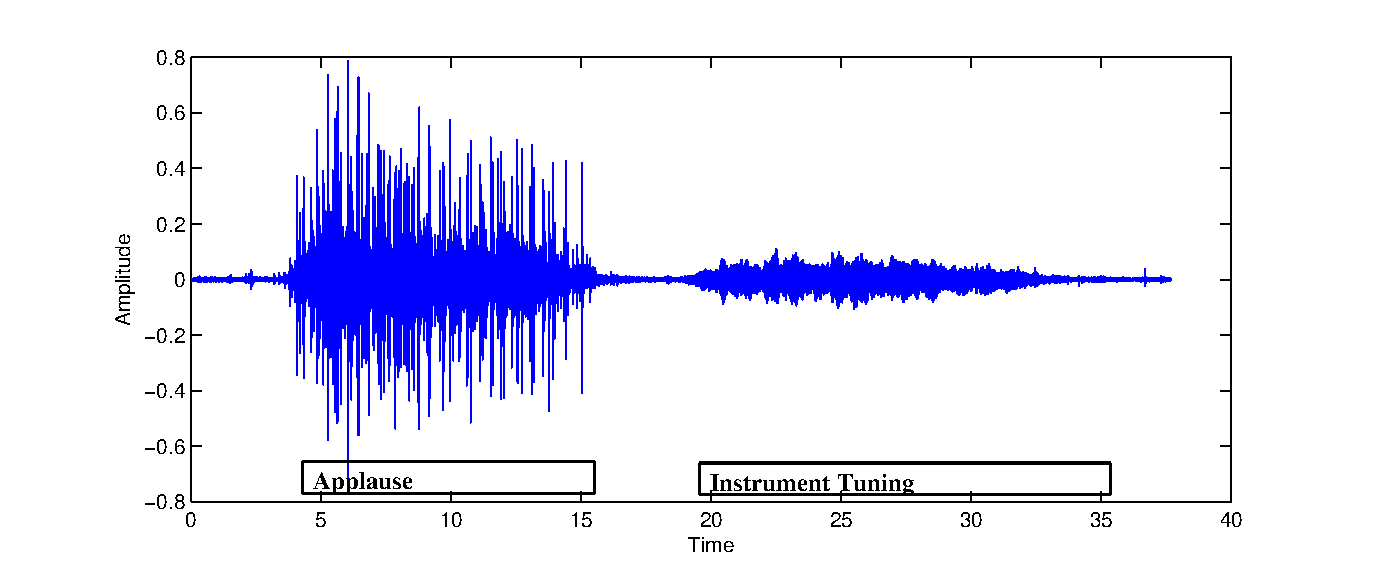
\includegraphics[scale=0.6]{figure/intro/waveform}
\caption{Waveform for a concert audio clip}
\label{fig:waveform}
\end{figure}

Figure \ref{fig:waveform} shows an example waveform for a concert environment. 
In this clip, two things happened. 
The first part of this waveform represents the sound when people are applauding. 
The second part is the sound when musicians are tuning their instruments. 
For a human, upon hearing these two things, we are easily to tell that this audio is recorded in a concert. 
And our problem throughout this thesis is to automatically detect out the events like \textit{applause} and \textit{instrument tuning}, 
and then to infer the scene \textit{concert} based on these two detected events. 

At here, we would like to give a detailed definition some terminology that we are going to use in this thesis. 

\section{Our Approach}
So in this thesis, we have proposed a system to automatically detect the events in an audio clip and then infer the scene or context from the detected audio events. 
We utilize a constructed audible event taxonomy, which helps us to categorize common audible events. 
Then Gaussian Mixture Models (GMMs) are built for modeling these audible events. 
We use audio data from Sound Search Engines where users can upload clips. 
The features we used for building GMMs are Mel-Frequency Cepstrum Coefficients (MFCCs). 
It is a popular feature for speech recognition, and we use it in our problem. 
In the scene recognition process, we first segment an audio clip by a segmenter, which uses frame energy and spectral centroid to calculate a threshold. 
After detecting for these segments, we use the relation we get from movie, play, TV series scripts to infer the scene of the original clip.  

\section{Thesis Organization}
The thesis is organizaed as follows: Chapter 2 gives a description about related works, in the area of audible events taxonomy, audio event detection and audio scene recognition. 
Chapter 3 reviews the data we used in this thesis, including event list and scene list. 
Then in chapter 4 we describes how event detection is carried out. 
Chapter 5 present the method we used to extract scene-event relations and scene recognition process. 
Evaluations of event detection and scene recognition are presented in chapter 6. 
Finally, chapter 7 gives a conclusion.   


%TC:fileinclude \import dir,file
\import{supplements/}{overview.tex}
%TC:fileinclude \subimport subdir,file
\subimport{tables/}{data.tex}
\end{lstlisting}


\subsection{Adding subcount break points}

By specifying \code{-sub}, \TeXcount{} can produce subcounts, e.g. per section. Alternatively, or in addition, explicit break points can be entered in the \LaTeX{} document using the TC-instruction \code{break}. These take the form:
\codeline{\%TC:break \textit{title}}
A title (or name) may be given to identify the break point.

If you define new section macros or macros you wish to cause a break point, these may be specified using the TC-instruction \code{breakmacro}:
\codeline{\%TC:breakmacro \textit{macro} \textit{label}}
This defines the given macro to cause a break point, and uses the given label to indicate the type of break (e.g. Section, Chapter, etc.).


\subsection{Ignoring segments of the file}

The TC-instruction \code{ignore}, later canceled by \code{endignore}, may be used to turn of all counting in a segment of the \LaTeX{} file. The ignored segment should thus be started by
\codeline{\%TC:ignore}
and ended by
\codeline{\%TC:endignore}
causing all text inbetween to be ignored.\footnote{In older versions, \TeXcount{} would still parse this text and might thus be affected by unbalanced braces. As of version 2.3, however, this should be fixed to make the ignore instruction more robust.}


\subsection{Bibliography inclusion}

In order to include the bibliography in the word counts, you can either specify \code{-incbib} on the command line, or use \TeXcount{} instruction
\codeline{\%TC:incbib}
which has the same effect: it specifies handling rules for the \code{\bs{bibliography}} macro and \code{thebibliography} environment that causes the bibliography to be included in the count, and if necessary the \code{.bbl} file to be included (without requiring \code{-inc} or \code{-merge}).


\subsection{Text substitution prior to parsing}

There are cases where a macro needs to be substituted with a text prior to parsing. One such case is when a macro contains a file path which is later used by a file inclusion macro. Since \TeXcount{} does not actually expand the macros, it will not be able to generate the file path from the macro. Instead, one may perform an explicit substitution
\codeline{\%TC:subst \parm{macro} \parm{text}}
which will then cause all occurrences of the macro to be substituted by the provided text prior to parsing. Note that this substitution will therefore also be found in the verbose output. 

\begin{lstlisting}
\newcommand\chappath{chapters}
%TC:subst \chappath chapters
\input \chappath/chapter1
\end{lstlisting}

Note that the substitution is placed \emph{after} the \code{\bs{newcommand}} definition. Otherwise, the substitution would have taken effect, changing that line to \code{\bs{newcommand} chapters/chapters}.



\subsection{Adding a new counter}

Initially, \TeXcount{} has eight different counters: file, text words, header words, other words, number of headers, number of floating objects, number of inlined formulae, and number of displayed formulae. However, it is possible to add more counters, e.g. to count footnotes separately. The syntax is
\codeline{\%TC:newcounter \parm{name} \opt{description}}
where the given name is used as keyword to refer to this counter. If no description is provided, the name will be used as description. A new counter is then added, and a parsing rule (parser state) with the same name is added which may be used in specifying macro and environment handling rules.

The following example shows how two different counters are added: one to count the number of footnotes, and another to count the words in footnote.

\begin{lstlisting}
%TC:newcounter fwords Words in footnotes
%TC:newcounter footnote Number of footnotes
%TC:macro \footnote [fwords]
%TC:macroword \footnote [footnote]
Each footnote\footnote{Words in footnotes will be counted separately.} will be counted.
\end{lstlisting}

Note that we have to specify one rule for counting the words in footnotes, and another rule for counting the footnotes. Unlike headers and floating bodies, there are no transition states available that can do both.


% ---------------------------------------------------------------------------

\section{Using an option file}

If you have a lot of settings, e.g. output template and TC commands for specifying parsing rules, you may place these into a file and include this using \code{-opt=\textit{file}}.

The format of this file is quite simple: each line is read as one option, so different options should not be placed on the same line. If some options are so long you need to break the line, e.g. for specifying an output template, you can do so by placing \code{\bs{}} at the start of lines that continue the previous line.

You may enter TC commands just as in the \LaTeX{} code by starting the line with \code{\%} instead of \code{TC:}. Using these, you may include specifications of parsing rules.

Blank lines and lines starting with \code{\#} are ignored and may thus be used to add comments to the option file. So are leading spaces, which allows lines to be indented. Line breaks may be inserted by \code{\bs{n}}.

Here is an example which sets the total sum to be the number of words (not including formulae), subcounts by section, parses included files, and adds an output template.

\begin{lstlisting}[frame=single]
### Options to use with TeXcount

# Counting options
-sum=1,1,1
-sub=section
-inc

# Macro rules
%macro \url 1
%envir sourcecode 0 0
%macroword \TeXcount 1

# Path used in file inclusion (\chapterpath filename)
%subst \chapterpath chap/

# Output template
-template=
   \::: {title} :::\n
   \Words: {sum}\n
   \Formulae: {6} + {7}\n
   \{5?Number of floats: {5}\n?5}
   \{SUB? - {sum} words in {title}\n?SUB}
\end{lstlisting}



% ---------------------------------------------------------------------------

\section{Customising \TeXcount{}}

\TeXcount{} is a self-contained Perl script: no external packages or resources required except that you need to have Perl installed to run it. Unfortunately, as with much of Perl code since Perl does not itself encourage structured programing, after expanding somewhat in size, it is not the most readable of codes. However, there may still be cases where you might yourself want to modify the code.

There are some things that may be modified quite easily even without knowing Perl.

\begin{description}

\item[Preset startup options]On one of the first lines of the code, the list \code{@StartupOptions} is defined. A list is simply a sequence of values (an array) on the form \code{(\textit{value},\textit{value},\ldots)}. As it stands, this list is empty, but you may add startup options to be included prior to command line options when you run \TeXcount{}. E.g. if you change this to \code{("-inc")} it will automatically add the \code{-inc} option so you don't have to do that yourself every time you run \TeXcount{}.

\item[Adding macro handling rules]While you may add macro handling rules using \code{\%TC:} commands either in the document or in a separate option file, this is inconvenient for large numbers of macros or if you want these rules always to be included. Also, you might want to add such rules for specific packages. In either case, it might be practical to add these directly to the \TeXcount{} code. \TeXcount{} stores the rules in hashes (maps from a key to a value) named \code{\%TeXmacro}, \code{\%TeXenvir}, etc. There is more documentation on each of these in the code itself, and you may also inspect how rules have been defined for other macros and environments.

\item[Output style]The ANSI colour codes for different levels of verbosity are encoded in the \code{\%STYLES} hashes and may be changed. The HTML style is encoded in the method \code{html_head()} and is easily modified. 

\item[Character and word definitions]\TeXcount{} identifies words as those that match one of a given set of regular expressions (defined in \code{@WordPatterns}). Note that \code{@WordPatterns} is changed by options \code{-chinese}, \code{-japanese} and  \code{-letters}. The pattern that is used within the word patterns to recognise letters is stored in \code{\$LetterPattern}. This is replaced if the \code{-relaxed} or \code{-restricted} option is set. Changing these definitions may be useful if you have special characters or wish to define words differently.

\end{description}


% ---------------------------------------------------------------------------

\section{Modifying the \TeXcount{} script}\label{sec:code}

\TeXcount{} is written in Perl, and although hardly the best structured and documented code ever seen, I have tried to structure and document it somewhat. In particular, some parts of the code should be easily modifiable even without in-depth knowledge of Perl or the \TeXcount{} script: e.g. the macro handling rules.

For more aid on how the \TeXcount{} script is coded and organised, please consult the Technical Documentation. However, here is a very brief overview:

\begin{description}

\item[Header and imports:] The shebang (\code{\#!}) and package imports (\code{use \parm{package}}).

\item[Global variables (and some methods related to these):] This defines and initialised global variables related to option settings, state variables used in parsing and counting (including functions for unterpreting these), variables and hashes for storing macro handling rules, and character class definitions (must be defined before use).

\item[Main program:] This simply contains a call to the \code{MAIN} routine with the command line arguments.

\item[Routines/functions/procedures:] The first procedure defined is \code{MAIN} which contains the program flow, then follows other subroutines. Routines with capitalised initial letters indicate high-level routines, while routines starting with underscores (\code{_}) are low-level routines.

\item[Text data:] At the end of the file is a \code{__DATA__} region containing text data used by the help routines.

\end{description}

Perl will first process the setup section which defines global variables, arrays and hashes. It then executes the main section (consisting of the call to \code{MAIN}), whereafter it exits. The subroutines and text data follow after the \code{exit}.



% ---------------------------------------------------------------------------

\section{License}

The \TeXcount{} package---script and accompanying documents---is distributed
under the \LaTeX{} Project Public License (LPPL)
\codeline{\url{http://www.latex-project.org/lppl.txt}}
which grants you, the user, the right to use, modify and distribute
the script. However, if the script is modified, you must change its
name or use other technical means to avoid confusion with the original script.


\end{document}
